\documentclass{standalone}
\usepackage{tikz}

\begin{document}
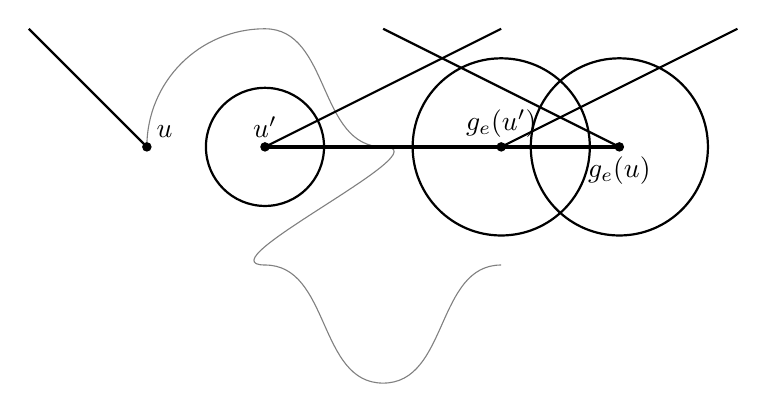
\begin{tikzpicture}[scale=1.5]
    % Define points
    \coordinate (u) at (-2,0);
    \coordinate (u_prime) at (-1,0);
    \coordinate (g_e_u_prime) at (1,0);
    \coordinate (g_e_u) at (2,0);

    % Original walk in gray
    \draw[gray] (u) to[out=90,in=180] ++(1,1) to[out=0,in=180] ++(1,-1) to[out=0,in=180] ++(-1,-1) to[out=0,in=180] ++(1,-1) to[out=0,in=180] ++(1,1);
    \filldraw (u) circle (1pt) node[above right] {$u$};
    
    % Modified walk in black
    \draw[ultra thick] (u_prime) -- (g_e_u_prime) -- (g_e_u);
    \filldraw (u_prime) circle (1pt) node[above] {$u'$};
    \filldraw (g_e_u_prime) circle (1pt) node[above] {$g_e(u')$};
    \filldraw (g_e_u) circle (1pt) node[below] {$g_e(u)$};

    % Draw circles around u', g_e(u'), and g_e(u)
    \draw[thick] (u_prime) circle (0.5);
    \draw[thick] (g_e_u_prime) circle (0.75);
    \draw[thick] (g_e_u) circle (0.75);

    % Additional paths for clarity
    \draw[thick] (-3,1) -- (u);
    \draw[thick] (u_prime) -- ++(2,1);
    \draw[thick] (g_e_u_prime) -- ++(2,1);
    \draw[thick] (g_e_u) -- ++(-2,1);
\end{tikzpicture}

\textit{Reflection-extension with splitting point $u$. The last part of the original walk is drawn in gray, the modified walk is drawn in black. Note that the distance between $u'$ and $g_e(u')$ is bounded by an absolute constant, so the increase in length will become negligible when the length of the original walk is large.}
\end{document}